\section{Super resolução de imagens}
\label{sec:sisr}

Super-resolução de imagens, é o processo de, artificialmente, produzir uma imagem de alta resolução a partir de uma imagem de baixa resolução. De acordo com \citeonline{nasrollahi_super-resolution_2014}, o objetivo da super-resolução de imagens, é aumentar a quantidade de \textit{pixels} por unidade de área em uma imagem, aumentando assim o nível de detalhes se compararmos o resultado, com a imagem original. Ainda de acordo com os autores citados anteriormente, inúmeras aplicações de super-resolução de imagens foram e são exploradas, e diversas técnicas para se performar a super-resolução de imagens são conhecidas hoje em dia. A figura \ref{fig:super-resolucao:fig11} abaixo, mostra as diferentes abordagens disponíveis para realizar super-resolução de imagens. 

\begin{figure}
    \centering
    \caption{Diagrama de diferentes áreas da super-resolução de imagens.}
    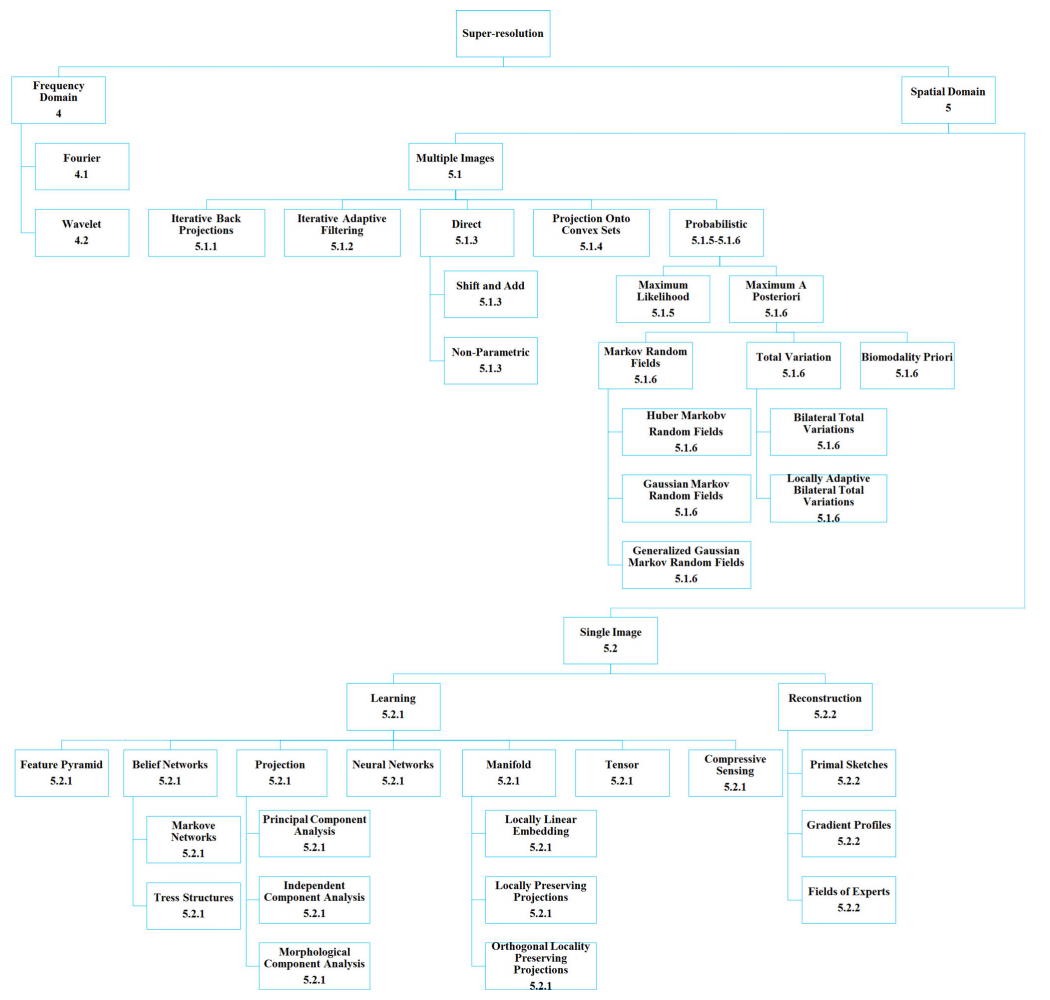
\includegraphics[width=11cm]{fig/SR-Taxidermy.png}
    \legend{Fonte: \cite{nasrollahi_super-resolution_2014}}
    \label{fig:super-resolucao:fig11}
\end{figure}

Como a imagem \ref{fig:super-resolucao:fig11} indica, a super-resolução de imagens, pode ser realizada utilizando diversos artifícios e algoritmos diferentes. Algumas das estratégias utilizadas para tal são rápidas e computacionalmente simples, como filtragem linear, bicúbica e Lanczos, porém produzem resultados de baixa qualidade \cite{ledig_photo-realistic_2016}. Estes métodos simplificam demasiadamente o problema de ampliar a resolução de uma imagem. Métodos envolvendo redes neurais convolucionais têm mostrado grande desempenho para a tarefa de aumentar a resolução de imagens \cite{ledig_photo-realistic_2016, dong_image_2015}. Estes métodos aprendem padrões espaciais das imagens de entrada, sendo capazes de extrair detalhes e características da imagem e aplicar nesta, o modelo. A figura \ref{fig:super-resolucao:fig14}, traz três exemplos de super-resolução: interpolação bicúbica, rede profunda residual e redes adversárias generativas, da esquerda para direita. Na extrema direita, está a imagem original, para fins de comparação.

\begin{figure}[H]
    \centering
    \caption{Diferentes métodos para super-resolução de imagens.}
    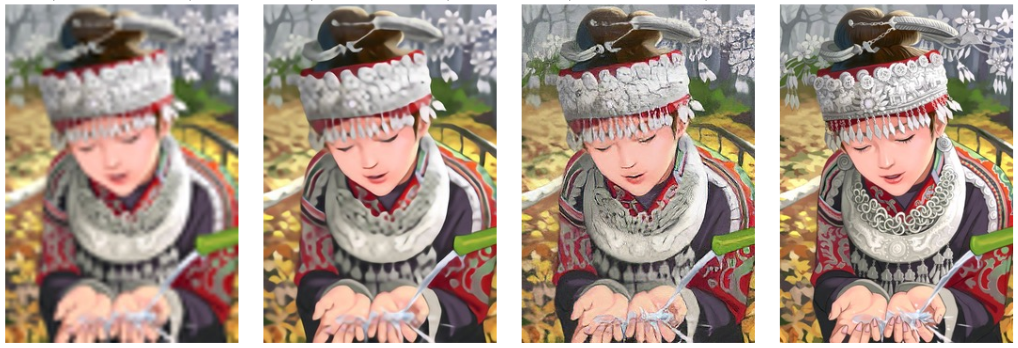
\includegraphics[width=12cm]{fig/SISR.png}
    \legend{Fonte: \cite{ledig_photo-realistic_2016}}
    \label{fig:super-resolucao:fig14}
\end{figure}
